\documentclass{report}
\usepackage{textcase}
\usepackage{amsmath}
\usepackage{amsfonts}
\usepackage{amssymb}
\usepackage[utf8]{vietnam}
\usepackage{graphicx}
\usepackage{scrextend}
\usepackage[left=3.5cm,right=2cm,top=3.5cm,bottom=3cm]{geometry}
\usepackage{xhfill}
\usepackage{floatrow}
\usepackage{subfigure}
\usepackage{wrapfig}
\usepackage{lipsum}
\usepackage{lettrine}
\usepackage[
    backend=biber,
    style=authoryear,
    natbib=true,
    url=true, 
    doi=true,
    eprint=false
]{biblatex}
\usepackage{hyperref} 
\addbibresource{myref.bib}

\begin{document}
\newcommand{\xfill}[2][1ex]{{%
  \dimen0=#2\advance\dimen0 by #1
  \leaders\hrule height \dimen0 depth -#1\hfill%
}}

%Page 1
\changefontsizes[14pt]{12pt}
\centerline{TỔNG LIÊN ĐOÀN LAO ĐỘNG VIỆT NAM}

\changefontsizes[14pt]{11pt}
\centerline{\textbf{TRƯỜNG ĐẠI HỌC TÔN ĐỨC THẮNG}}
\centerline{\textbf{KHOA CÔNG NGHỆ THÔNG TIN}}

\begin{center}
    \begin{figure}[htp]
    \begin{center}
     
\includegraphics[scale=.2]{logo}
    \end{center}
    \end{figure}
\end{center}

\changefontsizes{16pt}
\centerline{\textbf{BÀI TẬP LỚN: NHẬP MÔN HỆ ĐIỀU HÀNH}}
\vspace{1.5cm}
\changefontsizes{24pt}
\centerline{\textbf{GIẢI ĐÁP CÁC PROBLEM}}
\centerline{\textbf{CHƯƠNG 5 (PHẦN SỐ CHẴN)}}
\centerline{\textbf{MODERN OPERATING SYSTEMS}}

\vspace{4cm}
\begin{flushright}
\renewcommand{\baselinestretch}{0.05}
\changefontsizes{14pt}
\textit{Người hướng dẫn: }\textbf{G.V Trần Trung Tín}
\setlength{\parskip}{0.5em}

\textit{Người thực hiện: }\textbf{Trần Quốc Lĩnh - 51703124}
\setlength{\parskip}{0.5em}

Lớp: \textbf{17050301}
\setlength{\parskip}{0.5em}

Khoá: \textbf{21}
\setlength{\parskip}{0.5em}

\end{flushright}

\vspace{1cm}
\changefontsizes{14pt}
\centerline{\textbf{THÀNH PHỐ HỒ CHÍ MINH, NĂM 2018}}


%Page 2
\newpage
\changefontsizes[14pt]{12pt}
\centerline{TỔNG LIÊN ĐOÀN LAO ĐỘNG VIỆT NAM}

\changefontsizes[14pt]{11pt}
\centerline{\textbf{TRƯỜNG ĐẠI HỌC TÔN ĐỨC THẮNG}}
\centerline{\textbf{KHOA CÔNG NGHỆ THÔNG TIN}}

\begin{center}
    \begin{figure}[htp]
    \begin{center}
     
\includegraphics[scale=.2]{logo}
    \end{center}
    \end{figure}
\end{center}

\changefontsizes{16pt}
\centerline{\textbf{BÀI TẬP LỚN: NHẬP MÔN HỆ ĐIỀU HÀNH}}
\vspace{1.5cm}
\changefontsizes{24pt}
\centerline{\textbf{GIẢI ĐÁP CÁC PROBLEM}}
\centerline{\textbf{CHƯƠNG 5 (PHẦN SỐ CHẴN)}}
\centerline{\textbf{MODERN OPERATING SYSTEMS}}

\vspace{4cm}
\begin{flushright}
\renewcommand{\baselinestretch}{0.05}
\changefontsizes{14pt}
\textit{Người hướng dẫn: }\textbf{G.V Trần Trung Tín}
\setlength{\parskip}{0.5em}

\textit{Người thực hiện: }\textbf{Trần Quốc Lĩnh - 51703124}
\setlength{\parskip}{0.5em}

Lớp: \textbf{17050301}
\setlength{\parskip}{0.5em}

Khoá: \textbf{21}
\setlength{\parskip}{0.5em}

\end{flushright}

\vspace{1cm}
\changefontsizes{14pt}
\centerline{\textbf{THÀNH PHỐ HỒ CHÍ MINH, NĂM 2018}}


% Page 3
\newpage
\changefontsizes{16pt}
\centerline{\textbf{LỜI CẢM ƠN}}

\changefontsizes{13pt}
\bigskip
\setlength{\parindent}{2cm}

Cảm ơn thầy Trần Trung Tín đã tận tâm dạy môn nhập môn hệ điều hành, giúp em hiểu thế nào là hệ điều hành và cung cấp những kiến thức cần thiết để em làm bài tập lớn này!

Trong quá trình thực hiện bài tập lớn, em đã gặp không ít khó khăn. Cảm ơn thầy đã luôn dành thời gian quý báo của mình để tiếp sinh viên, để giúp những bạn như em giải quyết các khó khăn đó. Tuy nhiên vẫn không tránh khỏi những sai sót, em rất mong nhận được sự đánh giá và chỉ bảo từ thầy!
    
% Page 4
\newpage
\changefontsizes{16pt}
\centerline{\textbf{BÀI TẬP LỚN ĐƯỢC HOÀN THÀNH}}
\centerline{\textbf{TẠI TRƯỜNG ĐẠI HỌC TÔN ĐỨC THẮNG}}
\changefontsizes{13pt}
\vspace{1cm}
\setlength{\parindent}{2cm}
Em xin cam đoan đây là sản phẩm bài tập lớn của riêng em. Các nội dung nghiên cứu, kết quả trong đề tài này là trung thực và chưa công bố dưới bất kỳ hình thức nào trước đây. Những số liệu ,hình ảnh được chính em thu thập từ các nguồn khác nhau có ghi rõ trong phần tài liệu tham khảo.

\setlength{\parindent}{2cm}
Ngoài ra, trong bài tiểu luận còn sử dụng một số nhận xét, đánh giá cũng như số liệu của các tác giả khác, cơ quan tổ chức khác đều có trích dẫn và chú thích nguồn gốc.

\setlength{\parindent}{2cm}
Nếu phát hiện có bất kỳ sự gian lận nào em xin hoàn toàn chịu trách nhiệm về nội dung bài tập lớn của mình. Trường đại học Tôn Đức Thắng không liên quan đến những vi phạm tác quyền, bản quyền do em gây ra trong quá trình thực hiện (nếu có).

\vspace{0.75cm}
\begin{flushright}
\renewcommand{\baselinestretch}{0.05}
\changefontsizes{13pt}
\textit{TP. Hồ Chí Minh, ngày 10 tháng 10 năm 2018}
\end{flushright}

\setlength{\parindent}{13cm}
\textit{Tác giả }\\

\setlength{\parindent}{13cm}
\textit{(Đã ký)}\\

\setlength{\parindent}{12cm}
\textit{Trần Quốc Lĩnh}\\



% Page 5
\newpage
\changefontsizes{16pt}
\centerline{\textbf{PHẦN XÁC NHẬN VÀ ĐÁNH GIÁ CỦA GIẢNG VIÊN}}
\bigskip
\changefontsizes{13pt}
\setlength{\parindent}{2.2cm}
Phần xác nhận của GV hướng dẫn

\vspace{0.8cm}
\setlength{\parindent}{1cm}
\ \xfill{1pt} \

\bigskip
\ \xfill{1pt} \

\bigskip
\ \xfill{1pt} \

\bigskip
\ \xfill{1pt} \

\bigskip
\ \xfill{1pt} \

\bigskip
\ \xfill{1pt} \

\changefontsizes{12pt}
\setlength{\parindent}{8cm}
Tp. Hồ Chí Minh, ngày 10 tháng 10 năm 2018

\setlength{\parindent}{11cm}
\textit{(kí và ghi họ tên)}

\changefontsizes{13pt}
\vspace{2.5cm}
\setlength{\parindent}{2.2cm}
Phần đánh giá của GV chấm bài

\vspace{0.8cm}
\setlength{\parindent}{1cm}
\ \xfill{1pt} \

\bigskip
\ \xfill{1pt} \

\bigskip
\ \xfill{1pt} \

\bigskip
\ \xfill{1pt} \

\bigskip
\ \xfill{1pt} \

\bigskip
\ \xfill{1pt} \

\changefontsizes{12pt}
\setlength{\parindent}{8cm}
Tp. Hồ Chí Minh, ngày 10 tháng 10 năm 2018

\setlength{\parindent}{11cm}
\textit{(kí và ghi họ tên)}

% Page 6
\newpage
\changefontsizes{16pt}
\centerline{\textbf{TÓM TẮT}}\

\changefontsizes{13pt}
\setlength{\parindent}{2cm}
Với sự phát triển của thời đại kỹ thuật số, thì sở hữu một chiếc máy tính không còn là chuyện khó khăn nữa. Nhưng ít ai biết rằng để vận hành được một chiếc máy tính như thế đòi hỏi người ta phải tạo ra một chương trình, một hệ thống to lớn và phức tạp đến nhường nào. Bài tập lớn này sẽ trình bày một phần khá quan trọng trong hệ thống đồ sộ ấy, chính là \textbf{Input/Output}, thông qua việc giải quyết các problem (phần số chẵn) của chương 5, sách Modern operating systems.

Ngoài ra, em còn lên thư viện để tìm thêm thông tin để làm bài tập lớn vào các ngày 18/09, 02/10, 27/10, 30/10 và 05/11.

%Page 7
\newpage
\changefontsizes{16pt}
\centerline{\textbf{MỤC LỤC}}\

\vspace{1.2cm}
\changefontsizes{14pt}
\setlength{\parindent}{0cm}
LỜI CẢM ƠN\dotfill\ 3

\smallskip
CAM KẾT\dotfill\ 4

\smallskip
ĐÁNH GIÁ CỦA GIÁO VIÊN\dotfill\ 5

\smallskip
TÓM TẮT\dotfill\ 6

\smallskip
MỤC LỤC\dotfill\ 7

\smallskip
DANH MỤC CHÚ THÍCH CÁC THUẬT NGỮ VÀ HÌNH ẢNH\dotfill\ 8

\smallskip
GIẢI QUYẾT CÁC PROBLEM\\CHƯƠNG 5 - INPUT/OUTPUT (PHẦN SỐ CHẴN)\dotfill\ 10

TÀI LIỆU THAM KHẢO\dotfill\ 19

%Page 8
\newpage
\changefontsizes{16pt}
\centerline{\textbf{DANH MỤC CHÚ THÍCH CÁC THUẬT NGỮ}}
\centerline{\textbf{VÀ HÌNH ẢNH}}

\vspace{1cm}
\changefontsizes{14pt}
\textbf{Thuật ngữ}

\changefontsizes{13pt}
\bigskip
BitBlt : Là một data operation thường được sử dụng trong đồ họa máy tính, trong đó một số bitmap được kết hợp thành một hàm boolean.

\smallskip
Bitmap : Là một ánh xạ từ một số miền thành các bit. Nó cũng được gọi là một mảng các bit hoặc bitmap index.

\smallskip
Cylinder : Tập hợp các track được sắp theo cùng một thứ tự.

\smallskip
DMA : Là một cơ chế cho phép chuyển dữ liệu trực tiếp giữa các thiết bị nhập/xuất và RAM mà không cần thông qua CPU.

\smallskip
ECC : (Error-Correcting Code) được sử dụng để kiểm soát lỗi dữ liệu trên các kênh không đáng tin cậy hoặc dễ bị nhiễu.

\smallskip
Interrupt-driven : Mỗi ngắt có trình xử lí ngắt của riêng nó. Số lượng ngắt của phần cứng bị giới hạn với số yêu cầu ngắt tới bộ xử lí, nhưng có thể có hàng trăm phần mềm ngắt khác nhau. Ngắt là một kỹ thuật dùng trong đa nhiệm, đặc biệt là trong thời gian thực. Hệ thống như vậy được gọi là interrupt-driven.

\smallskip
I/O : (Input/output) nhập/xuất.

\smallskip
Level : Mức độ.

\smallskip
NVRAM : (Non-Volatile Random Access Memory) không bị mất dữ liệu khi tắt nguồn. NVRAM lưu trữ tất cả các thông tin mà hệ thống phải có trước lúc khởi động.

\smallskip
Overhead : Là sự kết hợp giữa sự thừa hoặc thời gian tính toán gián tiếp, bộ nhớ, băng thông hoặc các tài nguyên khác được yêu cầu để thực hiện một tác vụ cụ thể.

\smallskip
Program counter : Là thanh ghi bộ xử lý cho biết máy tính đang ở đâu trong chuỗi chương trình của nó.

\smallskip
PSW : (Program status word) là một hệ thống kế thừa kiến trúc IBM system/360 và thanh ghi điều khiển cho phép thực hiện chức năng của thanh ghi trạng thái và bộ đếm của chương trình trong các kiến trúc khác và hơn thế nữa.

\smallskip
RAID : (Redundant Arrays of Inexpensive Disks hoặc Redundant Arrays of Independent Disks) là hình thức ghép nhiều ổ đĩa cứng vật lý thành một hệ thống ổ đĩa cứng, có chức gia tăng tốc độ đọc/ghi dữ liệu, hoặc nhằm tăng thêm sự an toàn của dữ liệu chứa trên hệ thống đĩa, hoặc kết hợp cả hai yếu tố trên.

\smallskip
Parity : Chẵn lẻ.

\smallskip
RGB : Sử dụng mô hình ánh sáng bổ sung trong đó có ánh sáng đỏ (Red), xanh lục (Green) và xanh lam (Blue) được tổ hợp với nhau theo nhiều phương thức khác nhau để tạo thành các màu khác.

\smallskip
RPM : (Revolutions per minute) là số vòng quay/phút.

\smallskip
Sector : Là đơn vị format nhỏ nhất trên đĩa. 

\smallskip
Seek time : Thời gian di chuyển từ đầu đọc tới vị trí của dữ liệu trên đĩa.

\smallskip
SIGINT : Signals intelligence.

\smallskip
Stack : Ngăn xếp.

\smallskip
Track : Các vòng tròn trên đĩa.

\smallskip
Word : Một đơn vị dữ liệu kiểu word.

\changefontsizes{14pt}
\bigskip
\textbf{Hình ảnh}

\bigskip
\changefontsizes{13pt}
Hình 1 : Bảng liệt kê tốc độ của một số thiết bị, mạng và bus điển hình.

Hình 2 : Minh họa gián đoạn service procedure.

Hình 3 : Phân tích ảnh hưởng của sự cố đối với việc ghi ổn định


%Page ??
\newpage
\changefontsizes{16pt}
\centerline{\textbf{GIẢI QUYẾT CÁC PROBLEM}}
\centerline{\textbf{CHƯƠNG 5 - INPUT/OUTPUT (PHẦN SỐ CHẴN)}}

\bigskip
\setlength{\parindent}{0.0cm}
\changefontsizes{13pt}
\textbf{2. Với các tốc độ được liệt kê trong hình 5-1, có khả thi hay không khi quét (scan) tài liệu từ máy quét (scanner) và truyền chúng qua một mạng 802.11g với tốc độ tối đa?}

\begin{center}
     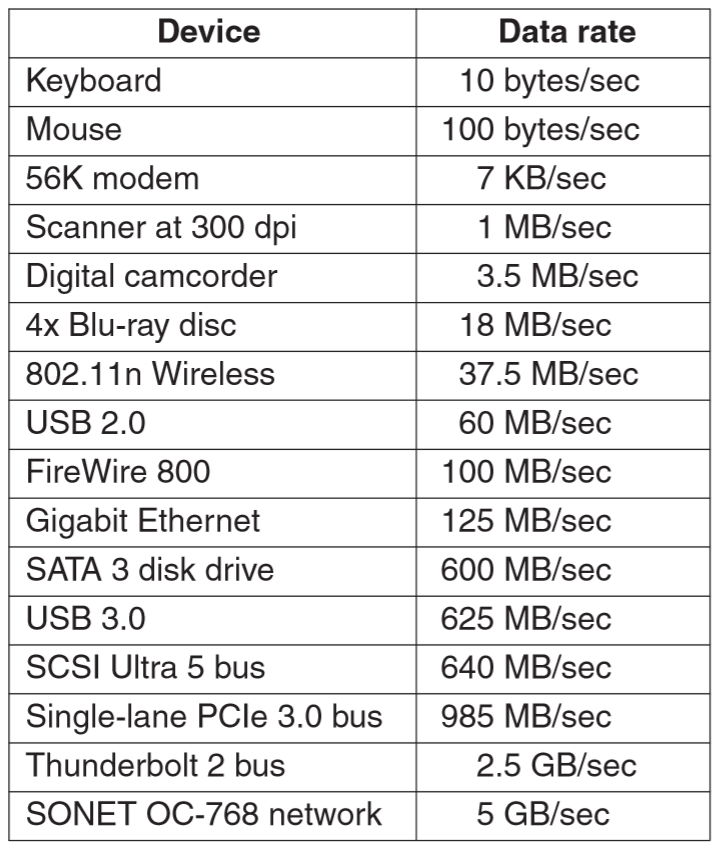
\includegraphics[scale=0.7]{hinh1}
\end{center}

\centerline{Hình 1 : Bảng liệt kê tốc độ của một số thiết bị, mạng và bus điển hình.}
\changefontsizes{12pt}
\centerline{Nguồn: Andrew S. Tanenbaum, Herbert Bos-Modern Operating Systems-Pearson (2014)}
\changefontsizes{13pt}

\bigskip
\textit{Trả lời:}

\smallskip
Khả thi! Vì máy quét (scanner) có tốc độ tối đa là 400KB/giây. Mà mạng không giây chạy ở tốc độ 6.75MB/giây nên sẽ không thành vấn đề khi truyền dữ liệu từ máy quét (scanner) qua mạng với tốc độ tối đa.

\bigskip
\textbf{4. Giải thích sự cân bằng giữa precise interrupt và imprecise interrupt trên máy superscalar.}

\bigskip
\textit{Trả lời:}

\smallskip
Imprecise interrupt làm cho code phức tạp, mà ưu thế của precise interrupt là sự đơn giản của code trong hệ điều hành vì trạng thái của máy cũng được xác định. Tuy nhiên, precise interrupt làm tăng độ phức tạp của thiết kế chip và vùng chip, điều này có thể khiến CPU chậm hơn.

\bigskip
\textbf{6. Giả sử rằng một hệ thống sử dụng DMA để truyền dữ liệu từ bộ điều khiển ổ đĩa sang bộ nhớ chính. Và giả sử trung bình mất t1 giây để kết nối được với các bus và t2 giây để chuyển một word qua bus (t1>>t2). Sau khi CPY đã được lập trình bộ điều khiển DMA, mất bao lâu để chuyển 1000 word từ bộ điều khiển ổ đĩa sang bộ nhớ chính, nếu\\
(a) Dùng chế độ word-at-a-time.\\
(b)	Dùng chế độ burst. Giả sử rằng việc ra lệnh cho bộ điều khiển ổ đĩa yêu cầu kết nối tới bus để gửi đi một word và thừa nhận một lần truyền dữ liệu cũng yêu cầu bus gửi đi một word.}

\bigskip
\textit{Trả lời:}

\smallskip
(a) Chế độ word-at-time:

\centerline{1000 $\times$ [(t1 + t2) + (t1 + t2) + (t1 + t2)]}
\changefontsizes{12pt}
\centerline{Nguồn: Andrew S. Tanenbaum, Herbert Bos-Modern Operating Systems-Pearson (2014).}
\changefontsizes{13pt}
\smallskip
Trong đó, phần đầu để kết nối với bus và gửi lệnh đến bộ điều khiển ổ đĩa, phần thứ hai để chuyển word, và phần thứ ba để được thừa nhận. Tất cả mất 3000 $\times$ (t1 + t2) nano giây.

\smallskip
(b) Chế dộ burst: 

\centerline{t1 + t2 + t1 + .... t2 + t1 + t2 (1000 lần)}
\changefontsizes{12pt}
\centerline{Nguồn: Andrew S. Tanenbaum, Herbert Bos-Modern Operating Systems-Pearson (2014).}
\changefontsizes{13pt}
\smallskip
Trong đó, phần đầu dùng để kết nối tới bus và gửi lệnh tới bộ điều khiển đĩa, phần hai dùng để bộ điều khiển đĩa kết nối tới bus, phần ba để chuyển burst, và phần bốn để kết nối với bus và thực hiện thừa nhận. Tất cả mất 3t1 + 1002t2.

\bigskip
\textbf{8. Giả sử rằng máy tính có thể đọc hoặc ghi một memory word trong 5 nano giây. Cũng giả sử rằng khi có một sự gián đoạn xảy ra, tất cả 32 thanh ghi CPU, cộng thêm program counter và PSW được đẩy lên stack. Cho biết số lượng tối đa gián đoạn/giây mà máy tính này có thể xử lí?}

\bigskip
\textit{Trả lời:}

\smallskip
Một gián đoạn yêu cầu đưa 34 word vào stack. Gián đoạn khác yêu cầu nạp 34 word từ stack. Nó overhead 340 nano giây. Do đó, máy tính có thể xử lí tối đa không hơn 2,94 triệu gián đoạn/giây.

\bigskip
\textbf{10. Trong hình 5-9(b), sự gián đoạn không được thừa nhận cho đến khi ký tự tiếp theo được đưa ra máy in. Nó có thể được thừa nhận ngay khi bắt đầu sự gián đoạn service procedure hay không? Nếu có, hãy đưa ra một lí do để làm điều đó ở bước cuối. Nếu không thì tại sao?}

\begin{center}
     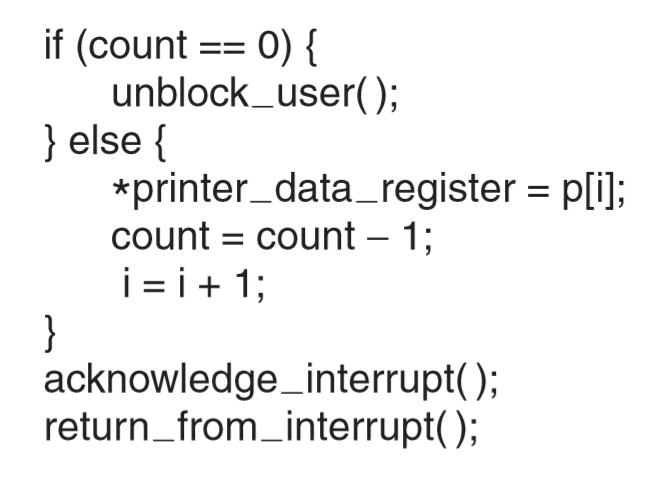
\includegraphics[scale=0.7]{hinh2}
\end{center}

\centerline{Hình 2 : Minh họa gián đoạn service procedure}
\changefontsizes{12pt}
\centerline{Nguồn: Andrew S. Tanenbaum, Herbert Bos-Modern Operating Systems-Pearson (2014)}
\changefontsizes{13pt}

\bigskip
\textit{Trả lời:}

\smallskip
Có! Là vì đoạn code cuối của gián đoạn service procedure rất ngắn. Bởi lần đầu xuất ra một ký tự khác và sau đó thừa nhận gián đoạn, nếu một gián đoạn khác xảy ra ngay lặp tức, máy in sẽ hoạt động suốt gián đoạn, làm cho nó in nhanh hơn một chút. Một bất lợi của phương pháp này là thời gian chết lâu hơn một chút khi các gián đoạn khác có thể bị vô hiệu hóa.


\bigskip
\textbf{12. Một trang văn bản thường gồm 50 dòng và 80 ký tự mỗi dòng. Tưởng tượng rằng một máy in có thể in 6 trang/phút và thời gian để ghi một ký tự vào thanh ghi output của máy in là quá ngắn mà nó có thể bị bỏ qua. Hợp lí hay không khi chạy máy in này bằng cách sử dụng interrupt-driven I/O nếu mỗi ký tự được in yêu cầu một gián đoạn mất 50 $\mu$ giây cho tất cả cho dịch vụ đó?}

\bigskip
\textit{Trả lời:}

\smallskip
Máy in in $50 \times 80 \times 6 = 24$ 000 ký tự/phút = 400 ký tự/giây. Mỗi ký tự sử dụng 50 $\mu$ giây của CPU cho mỗi gián đoạn, vì vậy cùng với mỗi gián đoạn overhead 20 mili giây. Sử dụng interrupt-driven I/O, thời gian còn lại là 980 mili giây sẵn có cho nhu cầu khác. Nói cách khác, gián đoạn overhead tốn 2\% của CPU, điều này hầu như không ảnh hưởng đến các chương trình đang chạy.

\bigskip
\textbf{14. Mỗi tác vụ dưới đây được thực thi ở đâu trong bốn tầng phần mềm I/O\\
(a) Tính toán track, sector và head cho việc đọc đĩa.\\
(b) Ghi lệnh vào thanh ghi của thiết bị.\\
(c)	Kiểm tra xem liệu người dùng có được phép sử dụng thiết bị.\\
(d) Chuyển đổi số nhị phân sang mã ASCII để in.}

\bigskip
\textit{Trả lời:}

\smallskip
(a) Trình điều khiển thiết bị.\\
(b) Trình điều khiển thiết bị.\\
(c) Phần mềm độc lập với phần cứng.\\
(d) Phần mềm người sử dụng.

\bigskip
\textbf{16. Tại sao tập tin output cho máy in thường được đặt trên đĩa trước khi được in ra?}

\bigskip
\textit{Trả lời:}

\smallskip
Nếu máy in được gán ngay khi có output, một tiến trình có thể kết nối với máy in ngày lặp tức bằng cách in một vài ký tự.\\

\bigskip
\textbf{18. Một đĩa quay tại 700 RPM. Nó có 500 sector của 512 byte xung quanh outer cylinder. Mất bao lâu để đọc một sector?}

\bigskip
\textit{Trả lời:}

\smallskip
Tại 700 RPM, tức là 120 vòng/giây, vì vậy mất khoảng 8.33 mili giây. Chia cho 500, ta có được khoảng 16,67 $\mu$ giây để đọc một sector.

\bigskip
\textbf{20. RAID level 3 có thể sửa lỗi bit đơn mà chỉ sử dụng một ổ đĩa parity. Còn RAID level 2 thì sao? Dù vậy, nó cũng chỉ có thể sửa chữa một lỗi duy nhất và tốn nhiều ổ đĩa để làm việc đó.}

\bigskip
\textit{Trả lời:}

\smallskip
RAID level 2 không chỉ có thể phục hồi từ các sự cố drive, mà còn từ các lỗi chưa được phát hiện. Nếu một drive hỏng một bit đơn duy nhất, RAID level 2 sẽ sửa lỗi này, mà RAID level 3 sẽ không.

\bigskip
\textbf{22. So sánh RAID từ level 0 đến 5 về phương diện hiệu suất đọc, ghi, space overhead và độ tin cậy.}

\bigskip
\textit{Trả lời:}

\smallskip
Hiệu suất đọc: Các RAID level 0, 2, 3, 4, và 5 cho phép đọc song song để phục vụ yêu cầu đọc. Tuy nhiên, RAID level 1 cho phép hơn 2 yêu cầu đọc thực hiện đồng thời.

\smallskip
Hiệu suất ghi: Tất cả level RAID đều cung cấp hiệu suất ghi như nhau.

\smallskip
Space overhead: Không có space overhead trong level 0 và 1. Với 32-bit dữ liệu word và sáu parity drive, space overhead là khoảng 18.75\% trong level 2, và 3.13\% ở level 3, 4 và 5.

\smallskip
Độ tin cậy: Không hỗ trợ độ tin cậy ở level 0. Tất cả các level còn lại có thể an toàn sau một sự cố ổ đĩa. Thêm nữa, trong level 3, 4, và 5, và một lỗi bit đơn ngẫu nhiên trong một word có thể được phát hiện, và còn có thể được sửa chữa trong level 2.

\bigskip
\textbf{24. Tại sao các thiết bị lưu trữ quang vốn vó khả năng chứa mật độ dữ liệu cao hơn các thiết bị lưu trữ từ tính?}

\bigskip
\textit{Trả lời:}

\smallskip
Khi một vùng từ trường được phát ra giữa hai cực. Không chỉ khó khăn ở việc làm cho nguồn của vùng từ trường nhỏ, mà còn phải phân tán nhanh chóng, dẫn đến các vấn đề cơ học là khá khó để giữ cho bề mặt của từ trường medium gần với nguồn từ trường hoặc cảm biến. Một laser bán dẫn phát ra được ánh sáng ở một vùng rất nhỏ, và áng sáng có thể được xử lí quang học để chiếu sáng ở một điểm rất nhỏ từ một khoảng cách tương đối lớn từ nguồn.

\bigskip
\textbf{26. Nếu bộ điều khiển ổ đĩa ghi các byte nó nhận được từ ổ đĩa vào bộ nhớ nhanh như cách nó nhận chúng, mà không có bộ đệm nội bộ nào, là xen kẽ hữu ích? Giải thích câu trả lời.}

\bigskip
\textit{Trả lời:}

\smallskip
Có thể. Nếu hầu hết các tập tin được lưu trữ trong các sector luận lí liên tục, nó có thể là xen kẽ hữu ích đối với các sector để cung cấp cho các chương trình thời gian xử lí dữ liệu vừa được nhận, vậy nên khi yêu cầu tiếp theo được đưa ra, ổ đĩa sẽ ở đúng nơi. Cho dù đây là vấn đề phụ thuộc chủ yếu vào loại chương trình và cách đồng bộ của chúng.

\bigskip
\textbf{28. Xét một đĩa từ gồm 16 head và 400 cylinder. Ổ đĩa này có bốn khu vực với 100 cylinder mỗi khu vực, bên trong chứa 160, 200, 240 và 280 sector tương ứng. Giả sử rằng mỗi secror chứa 512 byte, seek time trung bình giữa các cylinder liền kề là 1 mili giây, và ổ đĩa quay ở tốc độ 7200 RPM. Tính \\
(a) Dung lượng ổ đĩa\\
(b) Optimal track skew\\
(c) Tốc độ truyền dữ liệu tối đa.}

\bigskip
\textit{Trả lời:}

\smallskip
(a)Ta có:\centerline{Sức chứa của một vùng $ = track \times cylinder \times sector/cylinder \times byte/sec$}

\changefontsizes{11pt}
\centerline{Nguồn: Andrew S. Tanenbaum, Herbert Bos-Modern Operating Systems-Pearson (2014).}
\changefontsizes{13pt}



\setlength{\parindent}{1cm}
Sức chứa của vùng 1: $16 \times 100 \times 160 \times 512 = 131 072 000$ byte

Sức chứa của vùng 2: $16 \times 100 \times 200 \times 512 = 163 840 000$ byte

Sức chứa của vùng 3: $16 \times 100 \times 240 \times 512 = 196 608 000$ byte

Sức chứa của vùng 4: $16 \times 100 \times 280 \times 512 = 229 376 000$ byte

Tổng $= 131 072 000 + 163 840 000 + 196 608 000 229 376 000 = 720 896 000$ byte

\smallskip
\setlength{\parindent}{0cm}
(b) Tốc độ quay 7200 tức là 120 vòng/giây. Trong seek time track-to-track 1 mili giây, 0.12 của sector được cover.\\ Trong khu vực 1, head của ổ đĩa sẽ băng qua 0.12 $\times$ 160 sector trong 1 mili giây, vậy nên, optimal track skew đối với khu vực 1 là 19.2 sector.\\ Trong khu vực 2, head của ổ đĩa sẽ băng qua 0.12 $\times$ 200 sector trong 1 mili giây, vì vậy, optimal track skew đối với khu vực 2 là 24 sector.\\ Trong khu vực 3, head của ổ đĩa sẽ băng qua 0.12 x 240 sector trong 1 mili giây, vậy, optimal track skew dối với khu vực 3 là 28.8 sector.\\ Trong khu vực 4, head của ổ đĩa sẽ băng qua 0.12 $\times$ 280 sector trong 1 mili giây, nên, optimal track skew của khu vực 4 là 33.6 sector.

\smallskip
(c) Tốc độ truyền dữ liệu đạt tối đa là khi cylinder ở khu vực ngoài cùng (khu vực 4) đang được đọc/ghi. Trong khu vực đó, trong một giây, 280 sector được đọc 120 lần. Do đó, tốc độ truyền dữ liệu tối đa là $280 \times 120 \times 512 =$ 17 203 200 byte/giây.


\bigskip
\textbf{30. Một nhà sản xuất máy tính quyết định thiết kế lại bảng phân khu của đĩa cứng Pentium để cung cấp nhiều hơn bốn phân khu. Một số hệ quả của sự thay đổi này là?}

\bigskip
\textit{Trả lời:}

\smallskip
Một thực tế rõ khá ràng là không tồn tại hệ điều hành nào hoạt động được bởi chúng đều nhìn vào đó để xem các phân vùng ổ đĩa ở đâu. Thay đổi định dạng của bảng phân vùng sẽ khiến tất cả các hệ điều hành ngừng hoạt động. Chỉ có một cách duy nhất để thay đổi bảng phân vùng là đồng thời thay đổi tất cả các hệ điều hành để sử dụng định dạng mới.

\bigskip
\textbf{32. Một sửa đổi nhỏ của thuật toán thang máy đối với yêu cầu định thời ổ đĩa là luôn scan trong cùng một hướng. Thuật toán sửa đổi này có gì tốt hơn so với thuật toán thang máy?}

\bigskip
\textit{Trả lời:}

\smallskip
Trong trường hợp xấu nhất, một yêu cầu đọc/ghi không được đáp ứng cho gần hai lần scan toàn bộ ổ đĩa trong thuật toán thang máy, trong khi tối đa là một lần scan toàn bộ ổ đĩa cho thuật toán sửa đổi.

\bigskip
\textbf{34. Điều gì xảy ra nếu một sự cố xảy ra trước khi hệ điều hành kịp ghi lại một số block không hợp lệ trên NVRAM? Điều này có làm hỏng sự trừu tượng của ổn định lưu trữ? Giải thích?}

\bigskip
\textit{Trả lời:}

\smallskip
Không! Thực tế là một số thông tin chưa được ghi lại trên NVRAM làm cho chương trình phục hồi sẽ không biết block nào đã được ghi lại. Nó sẽ đọc cả hai bản copy, tìm điểm giống nhau giữa chúng, xem xét có sự thay đổi không, sau đó chọn 1 hành động chính xác. Ảnh hưởng của sự cố trước khi NVRAM được cập nhật chỉ làm cho chương trình phục hồi làm việc nhiều hơn cần thiết.

\bigskip
\textbf{36. Giả định rằng CPU làm hỏng một khu vực nào đó dẫn đến một ECC hoạt động không chính xác. Chuyện gì có thể phát sinh trong năm cơ chế phục hồi sự cố đã được trình bày ở hình 5-27 nếu giả thuyết này không đúng?}

\begin{center}
     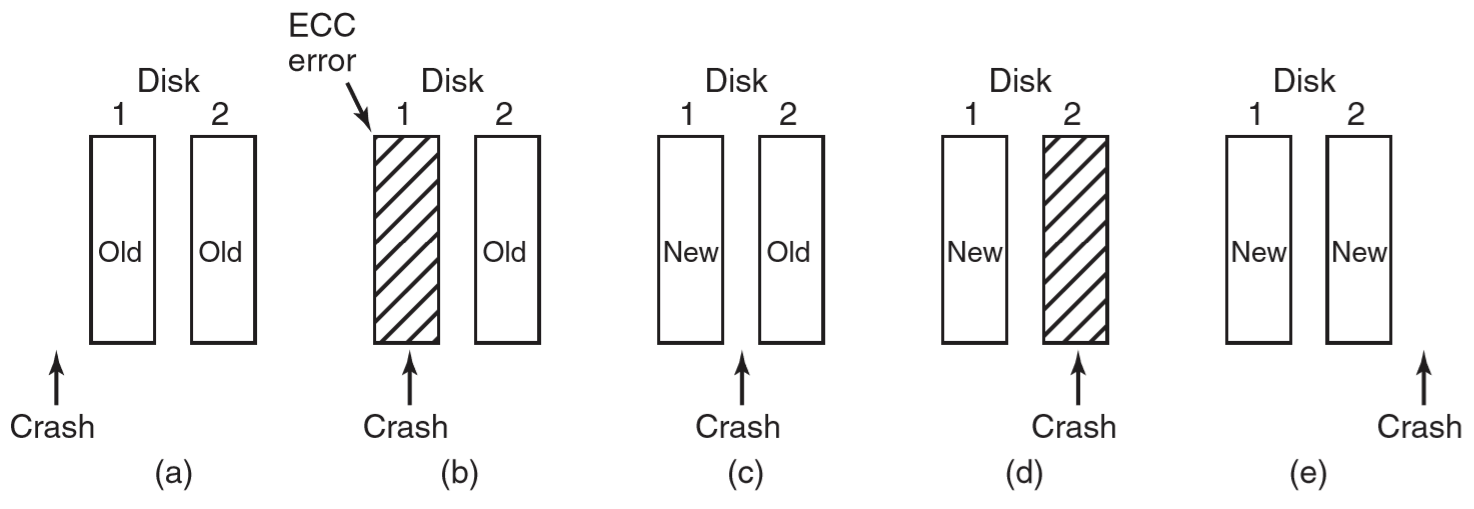
\includegraphics[scale=0.6]{hinh3}
\end{center}
\centerline{Hình 3 : Phân tích ảnh hưởng của sự cố đối với việc ghi ổn định}
\changefontsizes{12pt}
\centerline{Nguồn: Andrew S. Tanenbaum, Herbert Bos-Modern Operating Systems-Pearson (2014)}
\changefontsizes{13pt}

\bigskip
\textit{Trả lời:}

\smallskip
Nếu ECC thật sự hoạt động không chính xác, sẽ không thể phát hiện ở đĩa nào chứa lock hợp lệ (cũ hay mới), và cũng không thể phục hồi được dữ liệu.


\bigskip
\textbf{38. Một máy tính dùng một clock lập trình trong chế độ sóng vuông. Nếu dùng crystal 500 MHz, giá trị của thanh ghi là bao nhiêu để clock chuyển sang trạng thái khác mỗi\\
(a) Một mili giây (clock điểm từng mili giây)?\\
(b) 100 $\mu$ giây?}

\bigskip
\textit{Trả lời:}

\smallskip
Ta có:\\
(a) Sử dụng crystal 500 MHz, bộ đếm có thể giảm mỗi 2 nano giây. Nên, để điểm được mỗi mili giây, giá trị trên thanh ghi phải là 1 000 000/2 = 500 000.

\smallskip
(b) Để một clock điểm mỗi 100 $\mu$ giây, giá trị trên thanh ghi phải là 50 000.

\bigskip
\textbf{40. Nhiều phiên bản của UNIX sử dụng số nguyên 32-bit unsigned để theo dõi số giây kể từ thời gian gốc. Lần tiếp theo hệ thống wrap arround là khi nào (năm và tháng)? Điều này có khả năng xảy ra hay không?}

\bigskip
\textit{Trả lời:}

\smallskip
Số giây trong một năm: 365,25 $\times$ 24 $\times$ 3 600 = 31 557 600. Bộ đếm đã wrap arround sau 232 giây từ 1/1/1970. Vậy nên việc wrapping sẽ xảy ra tiếp theo khoảng 136,1 năm nữa tức là vào tháng 2 năm 2106. Và khi đó mỗi máy tính sẽ có ít nhất 64bit, vậy nên điều này không có khả năng xảy ra.

\bigskip
\textbf{42. Sau khi nhận được kí tự DEL (SIGNINT), trình điều khiển hiển thị loại bỏ tất cả output trong hàng đợi hiện tại cho hiển thị đó? Tại sao?}

\bigskip
\textit{Trả lời:}

\smallskip
Giả sử người dùng vô tình yêu cầu trình soạn thảo in hàng ngàn dòng. Sau đó, người dùng ấn DEL để dừng điều đó lại. Nếu trình điều khiển hiển thị không loại bỏ tất cả output trong hàng đợi ngay lặp tức sẽ khiến cho người dùng khó chịu khi không thấy có gì xảy ra và họ có thể sẽ ấn liên tục vào DEL.

\bigskip
\textbf{44. Các nhà thiết kế hệ thống máy tính mong đợi rằng những con chuột có thể di chuyển với tốc độ tối đa 20cm/giây. Nếu kích thước là 0.1 mm và mỗi con chuột truyền tin 3 byte, thì tốc độ truyền dữ liệu tối đa của con chuột là bao nhiêu? Giả định là mỗi con chuột được report một cách riêng biệt.}

\bigskip
\textit{Trả lời:}

\smallskip
Tốc độ tối đa mà chuột máy tính có thể di chuyển là 200mm/giây, tức là 2 000 mickey/giây. Nếu mỗi report là 3 byte, tốc độ đầu ra sẽ là 6 000 byte/giây.

\bigskip
\textbf{46. Một phương pháp để xếp chỗ một ký tự trên màn hình bitmap là sử dụng BitBlt từ bản phông chữ. Giả sử một phông chữ cụ thể sử dụng các ký tự có kích thước 16 x 24 pixel với mã màu RGB.\\
(a) Mỗi ký tự chiếm bao nhiêu không gian trên bản phông chữ?\\
(b) Nếu copy một byte mất 100 nano giây, bao gồm phần đầu, thì tốc độ output cho ra trên màn hình là bao nhiêu ký tự/giây?}

\bigskip
\textit{Trả lời:}

\smallskip
(a) Mỗi pixel tiêu tốn 3 byte trên mã màu RGB, nên không gian của bảng phải là 16 $\times$ 24 $\times$ 3 byte = 1 152 byte.

\smallskip
(b) Tại 100 nano giây mỗi byte, mỗi ký tự tiêu tốn 115,2 $\mu$ giây. Nên, tốc độ đầu ra là 8 681 ký tự/giây.



%Page ?? + 1
\newpage
\changefontsizes{16pt}
\centerline{\textbf{TÀI LIỆU THAM KHẢO}}

\vspace{1.2cm}
\changefontsizes{14pt}
\textbf{Tiếng Việt}

\vspace{1cm}
\url{https://vi.wikipedia.org/wiki/Bitmap}

\url{https://vi.wikipedia.org/wiki/C%C6%A1_ch%E1%BA%BF_DMA}

\url{https://vi.wikipedia.org/wiki/RAID}

\url{https://techgosu.com/nvram-la-gi-reset-nvram-khi-nao.html}

\vspace{3cm}
\textbf{Tiếng Anh}

\vspace{1cm}
\url{https://en.wikipedia.org/wiki/Input/output}

\url{https://en.wikipedia.org/wiki/Input%E2%80%93output_model}

\smallskip
Abraham Silberschatz, Peter B. Galvin, Greg Gagne, [2013], Operating System Concepts, 9th edition, Wiley.

Andrew S. Tanenbaum, Herbert Bos-Modern Operating Systems-Pearson (2014).

Operating Systems Design and Implementation (3rd Edition).


\end{document}